\documentclass[12pt]{article}
\usepackage{graphicx}
\graphicspath{{./images/}}

%packages
%\usepackage{latexsym}
\usepackage{graphicx}
\usepackage{color}
\usepackage{amsmath}
\usepackage{dsfont}
\usepackage{placeins}
\usepackage{amssymb}
\usepackage{wasysym}
\usepackage{abstract}
\usepackage{hyperref}
\usepackage{etoolbox}
\usepackage{datetime}
\usepackage{xcolor}
\usepackage{alphalph}
\settimeformat{ampmtime}

%\usepackage{pstricks,pst-node,pst-tree}

%\usepackage{algpseudocode}
%\usepackage{amsthm}
%\usepackage{hyperref}
%\usepackage{mathrsfs}
%\usepackage{amsfonts}
%\usepackage{bbding}
%\usepackage{listings}
%\usepackage{appendix}
\usepackage[margin=1in]{geometry}
%\geometry{papersize={8.5in,11in},total={6.5in,9in}}
%\usepackage{cancel}
%\usepackage{algorithmic, algorithm}

\makeatletter
\def\maxwidth{ %
  \ifdim\Gin@nat@width>\linewidth
    \linewidth
  \else
    \Gin@nat@width
  \fi
}
\makeatother

\definecolor{fgcolor}{rgb}{0.345, 0.345, 0.345}
\newcommand{\hlnum}[1]{\textcolor[rgb]{0.686,0.059,0.569}{#1}}%
\newcommand{\hlstr}[1]{\textcolor[rgb]{0.192,0.494,0.8}{#1}}%
\newcommand{\hlcom}[1]{\textcolor[rgb]{0.678,0.584,0.686}{\textit{#1}}}%
\newcommand{\hlopt}[1]{\textcolor[rgb]{0,0,0}{#1}}%
\newcommand{\hlstd}[1]{\textcolor[rgb]{0.345,0.345,0.345}{#1}}%
\newcommand{\hlkwa}[1]{\textcolor[rgb]{0.161,0.373,0.58}{\textbf{#1}}}%
\newcommand{\hlkwb}[1]{\textcolor[rgb]{0.69,0.353,0.396}{#1}}%
\newcommand{\hlkwc}[1]{\textcolor[rgb]{0.333,0.667,0.333}{#1}}%
\newcommand{\hlkwd}[1]{\textcolor[rgb]{0.737,0.353,0.396}{\textbf{#1}}}%

\usepackage{framed}
\makeatletter
\newenvironment{kframe}{%
 \def\at@end@of@kframe{}%
 \ifinner\ifhmode%
  \def\at@end@of@kframe{\end{minipage}}%
  \begin{minipage}{\columnwidth}%
 \fi\fi%
 \def\FrameCommand##1{\hskip\@totalleftmargin \hskip-\fboxsep
 \colorbox{shadecolor}{##1}\hskip-\fboxsep
     % There is no \\@totalrightmargin, so:
     \hskip-\linewidth \hskip-\@totalleftmargin \hskip\columnwidth}%
 \MakeFramed {\advance\hsize-\width
   \@totalleftmargin\z@ \linewidth\hsize
   \@setminipage}}%
 {\par\unskip\endMakeFramed%
 \at@end@of@kframe}
\makeatother

\definecolor{shadecolor}{rgb}{.77, .77, .77}
\definecolor{messagecolor}{rgb}{0, 0, 0}
\definecolor{warningcolor}{rgb}{1, 0, 1}
\definecolor{errorcolor}{rgb}{1, 0, 0}
\newenvironment{knitrout}{}{} % an empty environment to be redefined in TeX

\usepackage{alltt}
\usepackage[T1]{fontenc}

\newcommand{\qu}[1]{``#1''}
\newcounter{probnum}
\setcounter{probnum}{1}

%create definition to allow local margin changes
\def\changemargin#1#2{\list{}{\rightmargin#2\leftmargin#1}\item[]}
\let\endchangemargin=\endlist 

%allow equations to span multiple pages
\allowdisplaybreaks

%define colors and color typesetting conveniences
\definecolor{gray}{rgb}{0.5,0.5,0.5}
\definecolor{black}{rgb}{0,0,0}
\definecolor{white}{rgb}{1,1,1}
\definecolor{blue}{rgb}{0.5,0.5,1}
\newcommand{\inblue}[1]{\color{blue}#1 \color{black}}
\definecolor{green}{rgb}{0.133,0.545,0.133}
\newcommand{\ingreen}[1]{\color{green}#1 \color{black}}
\definecolor{yellow}{rgb}{1,1,0}
\newcommand{\inyellow}[1]{\color{yellow}#1 \color{black}}
\definecolor{orange}{rgb}{0.9,0.649,0}
\newcommand{\inorange}[1]{\color{orange}#1 \color{black}}
\definecolor{red}{rgb}{1,0.133,0.133}
\newcommand{\inred}[1]{\color{red}#1 \color{black}}
\definecolor{purple}{rgb}{0.58,0,0.827}
\newcommand{\inpurple}[1]{\color{purple}#1 \color{black}}
\definecolor{backgcode}{rgb}{0.97,0.97,0.8}
\definecolor{Brown}{cmyk}{0,0.81,1,0.60}
\definecolor{OliveGreen}{cmyk}{0.64,0,0.95,0.40}
\definecolor{CadetBlue}{cmyk}{0.62,0.57,0.23,0}

%define new math operators
\DeclareMathOperator*{\argmax}{arg\,max~}
\DeclareMathOperator*{\argmin}{arg\,min~}
\DeclareMathOperator*{\argsup}{arg\,sup~}
\DeclareMathOperator*{\arginf}{arg\,inf~}
\DeclareMathOperator*{\convolution}{\text{\Huge{$\ast$}}}
\newcommand{\infconv}[2]{\convolution^\infty_{#1 = 1} #2}
%true functions

%%%% GENERAL SHORTCUTS

%shortcuts for pure typesetting conveniences
\newcommand{\bv}[1]{\boldsymbol{#1}}

%shortcuts for compound constants
\newcommand{\BetaDistrConst}{\dfrac{\Gamma(\alpha + \beta)}{\Gamma(\alpha)\Gamma(\beta)}}
\newcommand{\NormDistrConst}{\dfrac{1}{\sqrt{2\pi\sigma^2}}}

%shortcuts for conventional symbols
\newcommand{\tsq}{\tau^2}
\newcommand{\tsqh}{\hat{\tau}^2}
\newcommand{\sigsq}{\sigma^2}
\newcommand{\sigsqsq}{\parens{\sigma^2}^2}
\newcommand{\sigsqovern}{\dfrac{\sigsq}{n}}
\newcommand{\tausq}{\tau^2}
\newcommand{\tausqalpha}{\tau^2_\alpha}
\newcommand{\tausqbeta}{\tau^2_\beta}
\newcommand{\tausqsigma}{\tau^2_\sigma}
\newcommand{\betasq}{\beta^2}
\newcommand{\sigsqvec}{\bv{\sigma}^2}
\newcommand{\sigsqhat}{\hat{\sigma}^2}
\newcommand{\sigsqhatmlebayes}{\sigsqhat_{\text{Bayes, MLE}}}
\newcommand{\sigsqhatmle}[1]{\sigsqhat_{#1, \text{MLE}}}
\newcommand{\bSigma}{\bv{\Sigma}}
\newcommand{\bSigmainv}{\bSigma^{-1}}
\newcommand{\thetavec}{\bv{\theta}}
\newcommand{\thetahat}{\hat{\theta}}
\newcommand{\thetahatmle}{\hat{\theta}_{\mathrm{MLE}}}
\newcommand{\thetavechatmle}{\hat{\thetavec}_{\mathrm{MLE}}}
\newcommand{\muhat}{\hat{\mu}}
\newcommand{\musq}{\mu^2}
\newcommand{\muvec}{\bv{\mu}}
\newcommand{\muhatmle}{\muhat_{\text{MLE}}}
\newcommand{\lambdahat}{\hat{\lambda}}
\newcommand{\lambdahatmle}{\lambdahat_{\text{MLE}}}
\newcommand{\etavec}{\bv{\eta}}
\newcommand{\alphavec}{\bv{\alpha}}
\newcommand{\minimaxdec}{\delta^*_{\mathrm{mm}}}
\newcommand{\ybar}{\bar{y}}
\newcommand{\xbar}{\bar{x}}
\newcommand{\Xbar}{\bar{X}}
\newcommand{\phat}{\hat{p}}
\newcommand{\Phat}{\hat{P}}
\newcommand{\Zbar}{\bar{Z}}
\newcommand{\iid}{~{\buildrel iid \over \sim}~}
\newcommand{\inddist}{~{\buildrel ind \over \sim}~}
\newcommand{\approxdist}{~{\buildrel approx \over \sim}~}
\newcommand{\equalsindist}{~{\buildrel d \over =}~}
\newcommand{\loglik}[1]{\ell\parens{#1}}
\newcommand{\thetahatkminone}{\thetahat^{(k-1)}}
\newcommand{\thetahatkplusone}{\thetahat^{(k+1)}}
\newcommand{\thetahatk}{\thetahat^{(k)}}
\newcommand{\half}{\frac{1}{2}}
\newcommand{\third}{\frac{1}{3}}
\newcommand{\twothirds}{\frac{2}{3}}
\newcommand{\fourth}{\frac{1}{4}}
\newcommand{\fifth}{\frac{1}{5}}
\newcommand{\sixth}{\frac{1}{6}}

%shortcuts for vector and matrix notation
\newcommand{\A}{\bv{A}}
\newcommand{\At}{\A^T}
\newcommand{\Ainv}{\inverse{\A}}
\newcommand{\B}{\bv{B}}
\newcommand{\K}{\bv{K}}
\newcommand{\Kt}{\K^T}
\newcommand{\Kinv}{\inverse{K}}
\newcommand{\Kinvt}{(\Kinv)^T}
\newcommand{\M}{\bv{M}}
\newcommand{\Bt}{\B^T}
\newcommand{\Q}{\bv{Q}}
\newcommand{\Qt}{\Q^T}
\newcommand{\R}{\bv{R}}
\newcommand{\Rt}{\R^T}
\newcommand{\Z}{\bv{Z}}
\newcommand{\X}{\bv{X}}
\newcommand{\Xsub}{\X_{\text{(sub)}}}
\newcommand{\Xsubadj}{\X_{\text{(sub,adj)}}}
\newcommand{\I}{\bv{I}}
\newcommand{\Y}{\bv{Y}}
\newcommand{\sigsqI}{\sigsq\I}
\renewcommand{\P}{\bv{P}}
\newcommand{\Psub}{\P_{\text{(sub)}}}
\newcommand{\Pt}{\P^T}
\newcommand{\Pii}{P_{ii}}
\newcommand{\Pij}{P_{ij}}
\newcommand{\IminP}{(\I-\P)}
\newcommand{\Xt}{\bv{X}^T}
\newcommand{\XtX}{\Xt\X}
\newcommand{\XtXinv}{\parens{\Xt\X}^{-1}}
\newcommand{\XtXinvXt}{\XtXinv\Xt}
\newcommand{\XXtXinvXt}{\X\XtXinvXt}
\newcommand{\x}{\bv{x}}
\newcommand{\onevec}{\bv{1}}
\newcommand{\oneton}{1, \ldots, n}
\newcommand{\yoneton}{y_1, \ldots, y_n}
\newcommand{\yonetonorder}{y_{(1)}, \ldots, y_{(n)}}
\newcommand{\Yoneton}{Y_1, \ldots, Y_n}
\newcommand{\iinoneton}{i \in \braces{\oneton}}
\newcommand{\onetom}{1, \ldots, m}
\newcommand{\jinonetom}{j \in \braces{\onetom}}
\newcommand{\xoneton}{x_1, \ldots, x_n}
\newcommand{\Xoneton}{X_1, \ldots, X_n}
\newcommand{\xt}{\x^T}
\newcommand{\y}{\bv{y}}
\newcommand{\yt}{\y^T}
\renewcommand{\c}{\bv{c}}
\newcommand{\ct}{\c^T}
\newcommand{\tstar}{\bv{t}^*}
\renewcommand{\u}{\bv{u}}
\renewcommand{\v}{\bv{v}}
\renewcommand{\a}{\bv{a}}
\newcommand{\s}{\bv{s}}
\newcommand{\yadj}{\y_{\text{(adj)}}}
\newcommand{\xjadj}{\x_{j\text{(adj)}}}
\newcommand{\xjadjM}{\x_{j \perp M}}
\newcommand{\yhat}{\hat{\y}}
\newcommand{\yhatsub}{\yhat_{\text{(sub)}}}
\newcommand{\yhatstar}{\yhat^*}
\newcommand{\yhatstarnew}{\yhatstar_{\text{new}}}
\newcommand{\z}{\bv{z}}
\newcommand{\zt}{\z^T}
\newcommand{\bb}{\bv{b}}
\newcommand{\bbt}{\bb^T}
\newcommand{\bbeta}{\bv{\beta}}
\newcommand{\beps}{\bv{\epsilon}}
\newcommand{\bepst}{\beps^T}
\newcommand{\e}{\bv{e}}
\newcommand{\Mofy}{\M(\y)}
\newcommand{\KofAlpha}{K(\alpha)}
\newcommand{\ellset}{\mathcal{L}}
\newcommand{\oneminalph}{1-\alpha}
\newcommand{\SSE}{\text{SSE}}
\newcommand{\SSEsub}{\text{SSE}_{\text{(sub)}}}
\newcommand{\MSE}{\text{MSE}}
\newcommand{\RMSE}{\text{RMSE}}
\newcommand{\SSR}{\text{SSR}}
\newcommand{\SST}{\text{SST}}
\newcommand{\JSest}{\delta_{\text{JS}}(\x)}
\newcommand{\Bayesest}{\delta_{\text{Bayes}}(\x)}
\newcommand{\EmpBayesest}{\delta_{\text{EmpBayes}}(\x)}
\newcommand{\BLUPest}{\delta_{\text{BLUP}}}
\newcommand{\MLEest}[1]{\hat{#1}_{\text{MLE}}}

%shortcuts for Linear Algebra stuff (i.e. vectors and matrices)
\newcommand{\twovec}[2]{\bracks{\begin{array}{c} #1 \\ #2 \end{array}}}
\newcommand{\threevec}[3]{\bracks{\begin{array}{c} #1 \\ #2 \\ #3 \end{array}}}
\newcommand{\fivevec}[5]{\bracks{\begin{array}{c} #1 \\ #2 \\ #3 \\ #4 \\ #5 \end{array}}}
\newcommand{\twobytwomat}[4]{\bracks{\begin{array}{cc} #1 & #2 \\ #3 & #4 \end{array}}}
\newcommand{\threebytwomat}[6]{\bracks{\begin{array}{cc} #1 & #2 \\ #3 & #4 \\ #5 & #6 \end{array}}}

%shortcuts for conventional compound symbols
\newcommand{\thetainthetas}{\theta \in \Theta}
\newcommand{\reals}{\mathbb{R}}
\newcommand{\complexes}{\mathbb{C}}
\newcommand{\rationals}{\mathbb{Q}}
\newcommand{\integers}{\mathbb{Z}}
\newcommand{\naturals}{\mathbb{N}}
\newcommand{\forallninN}{~~\forall n \in \naturals}
\newcommand{\forallxinN}[1]{~~\forall #1 \in \reals}
\newcommand{\matrixdims}[2]{\in \reals^{\,#1 \times #2}}
\newcommand{\inRn}[1]{\in \reals^{\,#1}}
\newcommand{\mathimplies}{\quad\Rightarrow\quad}
\newcommand{\mathlogicequiv}{\quad\Leftrightarrow\quad}
\newcommand{\eqncomment}[1]{\quad \text{(#1)}}
\newcommand{\limitn}{\lim_{n \rightarrow \infty}}
\newcommand{\limitN}{\lim_{N \rightarrow \infty}}
\newcommand{\limitd}{\lim_{d \rightarrow \infty}}
\newcommand{\limitt}{\lim_{t \rightarrow \infty}}
\newcommand{\limitsupn}{\limsup_{n \rightarrow \infty}~}
\newcommand{\limitinfn}{\liminf_{n \rightarrow \infty}~}
\newcommand{\limitk}{\lim_{k \rightarrow \infty}}
\newcommand{\limsupn}{\limsup_{n \rightarrow \infty}}
\newcommand{\limsupk}{\limsup_{k \rightarrow \infty}}
\newcommand{\floor}[1]{\left\lfloor #1 \right\rfloor}
\newcommand{\ceil}[1]{\left\lceil #1 \right\rceil}

%shortcuts for environments
\newcommand{\beqn}{\vspace{-0.25cm}\begin{eqnarray*}}
\newcommand{\eeqn}{\end{eqnarray*}}
\newcommand{\bneqn}{\vspace{-0.25cm}\begin{eqnarray}}
\newcommand{\eneqn}{\end{eqnarray}}

%shortcuts for mini environments
\newcommand{\parens}[1]{\left(#1\right)}
\newcommand{\squared}[1]{\parens{#1}^2}
\newcommand{\tothepow}[2]{\parens{#1}^{#2}}
\newcommand{\prob}[1]{\mathbb{P}\parens{#1}}
\newcommand{\cprob}[2]{\prob{#1~|~#2}}
\newcommand{\littleo}[1]{o\parens{#1}}
\newcommand{\bigo}[1]{O\parens{#1}}
\newcommand{\Lp}[1]{\mathbb{L}^{#1}}
\renewcommand{\arcsin}[1]{\text{arcsin}\parens{#1}}
\newcommand{\prodonen}[2]{\bracks{\prod_{#1=1}^n #2}}
\newcommand{\mysum}[4]{\sum_{#1=#2}^{#3} #4}
\newcommand{\sumonen}[2]{\sum_{#1=1}^n #2}
\newcommand{\infsum}[2]{\sum_{#1=1}^\infty #2}
\newcommand{\infprod}[2]{\prod_{#1=1}^\infty #2}
\newcommand{\infunion}[2]{\bigcup_{#1=1}^\infty #2}
\newcommand{\infinter}[2]{\bigcap_{#1=1}^\infty #2}
\newcommand{\infintegral}[2]{\int^\infty_{-\infty} #2 ~\text{d}#1}
\newcommand{\supthetas}[1]{\sup_{\thetainthetas}\braces{#1}}
\newcommand{\bracks}[1]{\left[#1\right]}
\newcommand{\braces}[1]{\left\{#1\right\}}
\newcommand{\set}[1]{\left\{#1\right\}}
\newcommand{\abss}[1]{\left|#1\right|}
\newcommand{\norm}[1]{\left|\left|#1\right|\right|}
\newcommand{\normsq}[1]{\norm{#1}^2}
\newcommand{\inverse}[1]{\parens{#1}^{-1}}
\newcommand{\rowof}[2]{\parens{#1}_{#2\cdot}}

%shortcuts for functionals
\newcommand{\realcomp}[1]{\text{Re}\bracks{#1}}
\newcommand{\imagcomp}[1]{\text{Im}\bracks{#1}}
\newcommand{\range}[1]{\text{range}\bracks{#1}}
\newcommand{\colsp}[1]{\text{colsp}\bracks{#1}}
\newcommand{\rowsp}[1]{\text{rowsp}\bracks{#1}}
\newcommand{\tr}[1]{\text{tr}\bracks{#1}}
\newcommand{\rank}[1]{\text{rank}\bracks{#1}}
\newcommand{\proj}[2]{\text{Proj}_{#1}\bracks{#2}}
\newcommand{\projcolspX}[1]{\text{Proj}_{\colsp{\X}}\bracks{#1}}
\newcommand{\median}[1]{\text{median}\bracks{#1}}
\newcommand{\mean}[1]{\text{mean}\bracks{#1}}
\newcommand{\dime}[1]{\text{dim}\bracks{#1}}
\renewcommand{\det}[1]{\text{det}\bracks{#1}}
\newcommand{\expe}[1]{\mathbb{E}\bracks{#1}}
\newcommand{\expeabs}[1]{\expe{\abss{#1}}}
\newcommand{\expesub}[2]{\mathbb{E}_{#1}\bracks{#2}}
\newcommand{\indic}[1]{\mathds{1}_{#1}}
\newcommand{\var}[1]{\mathbb{V}\text{ar}\bracks{#1}}
\newcommand{\cov}[2]{\mathbb{C}\text{ov}\bracks{#1, #2}}
\newcommand{\corr}[2]{\text{Corr}\bracks{#1, #2}}
\newcommand{\se}[1]{\mathbb{S}\text{E}\bracks{#1}}
\newcommand{\seest}[1]{\hat{\mathbb{S}\text{E}}\bracks{#1}}
\newcommand{\bias}[1]{\text{Bias}\bracks{#1}}
\newcommand{\derivop}[2]{\dfrac{\text{d}}{\text{d} #1}\bracks{#2}}
\newcommand{\partialop}[2]{\dfrac{\partial}{\partial #1}\bracks{#2}}
\newcommand{\secpartialop}[2]{\dfrac{\partial^2}{\partial #1^2}\bracks{#2}}
\newcommand{\mixpartialop}[3]{\dfrac{\partial^2}{\partial #1 \partial #2}\bracks{#3}}

%shortcuts for functions
\renewcommand{\exp}[1]{\mathrm{exp}\parens{#1}}
\renewcommand{\cos}[1]{\text{cos}\parens{#1}}
\renewcommand{\sin}[1]{\text{sin}\parens{#1}}
\newcommand{\sign}[1]{\text{sign}\parens{#1}}
\newcommand{\are}[1]{\mathrm{ARE}\parens{#1}}
\newcommand{\natlog}[1]{\ln\parens{#1}}
\newcommand{\oneover}[1]{\frac{1}{#1}}
\newcommand{\overtwo}[1]{\frac{#1}{2}}
\newcommand{\overn}[1]{\frac{#1}{n}}
\newcommand{\oneoversqrt}[1]{\oneover{\sqrt{#1}}}
\newcommand{\sqd}[1]{\parens{#1}^2}
\newcommand{\loss}[1]{\ell\parens{\theta, #1}}
\newcommand{\losstwo}[2]{\ell\parens{#1, #2}}
\newcommand{\cf}{\phi(t)}

%English language specific shortcuts
\newcommand{\ie}{\textit{i.e.} }
\newcommand{\AKA}{\textit{AKA} }
\renewcommand{\iff}{\textit{iff}}
\newcommand{\eg}{\textit{e.g.} }
\newcommand{\st}{\textit{s.t.} }
\newcommand{\wrt}{\textit{w.r.t.} }
\newcommand{\mathst}{~~\text{\st}~~}
\newcommand{\mathand}{~~\text{and}~~}
\newcommand{\ala}{\textit{a la} }
\newcommand{\ppp}{posterior predictive p-value}
\newcommand{\dd}{dataset-to-dataset}

%shortcuts for distribution titles
\newcommand{\logistic}[2]{\mathrm{Logistic}\parens{#1,\,#2}}
\newcommand{\bernoulli}[1]{\mathrm{Bernoulli}\parens{#1}}
\newcommand{\betanot}[2]{\mathrm{Beta}\parens{#1,\,#2}}
\newcommand{\stdbetanot}{\betanot{\alpha}{\beta}}
\newcommand{\betabinomial}[3]{\text{BetaBinomial}\parens{#1,\,#2,\,#3}}
\newcommand{\multnormnot}[3]{\mathcal{N}_{#1}\parens{#2,\,#3}}
\newcommand{\normnot}[2]{\mathcal{N}\parens{#1,\,#2}}
\newcommand{\classicnormnot}{\normnot{\mu}{\sigsq}}
\newcommand{\stdnormnot}{\normnot{0}{1}}
\newcommand{\uniformdiscrete}[1]{\mathrm{Uniform}\parens{\braces{#1}}}
\newcommand{\uniform}[2]{\mathrm{U}\parens{#1,\,#2}}
\newcommand{\stduniform}{\uniform{0}{1}}
\newcommand{\geometric}[1]{\mathrm{Geometric}\parens{#1}}
\newcommand{\hypergeometric}[3]{\mathrm{Hypergeometric}\parens{#1,\,#2,\,#3}}
\newcommand{\exponential}[1]{\mathrm{Exp}\parens{#1}}
\newcommand{\gammadist}[2]{\mathrm{Gamma}\parens{#1, #2}}
\newcommand{\poisson}[1]{\mathrm{Poisson}\parens{#1}}
\newcommand{\binomial}[2]{\mathrm{Binomial}\parens{#1,\,#2}}
\newcommand{\negbin}[2]{\mathrm{NegBin}\parens{#1,\,#2}}
\newcommand{\rayleigh}[1]{\mathrm{Rayleigh}\parens{#1}}
\newcommand{\multinomial}[2]{\mathrm{Multinomial}\parens{#1,\,#2}}
\newcommand{\gammanot}[2]{\mathrm{Gamma}\parens{#1,\,#2}}
\newcommand{\cauchynot}[2]{\text{Cauchy}\parens{#1,\,#2}}
\newcommand{\invchisqnot}[1]{\text{Inv}\chisq{#1}}
\newcommand{\invscaledchisqnot}[2]{\text{ScaledInv}\ncchisq{#1}{#2}}
\newcommand{\invgammanot}[2]{\text{InvGamma}\parens{#1,\,#2}}
\newcommand{\chisq}[1]{\chi^2_{#1}}
\newcommand{\ncchisq}[2]{\chi^2_{#1}\parens{#2}}
\newcommand{\ncF}[3]{F_{#1,#2}\parens{#3}}

%shortcuts for PDF's of common distributions
\newcommand{\logisticpdf}[3]{\oneover{#3}\dfrac{\exp{-\dfrac{#1 - #2}{#3}}}{\parens{1+\exp{-\dfrac{#1 - #2}{#3}}}^2}}
\newcommand{\betapdf}[3]{\dfrac{\Gamma(#2 + #3)}{\Gamma(#2)\Gamma(#3)}#1^{#2-1} (1-#1)^{#3-1}}
\newcommand{\normpdf}[3]{\frac{1}{\sqrt{2\pi#3}}\exp{-\frac{1}{2#3}(#1 - #2)^2}}
\newcommand{\normpdfvarone}[2]{\dfrac{1}{\sqrt{2\pi}}e^{-\half(#1 - #2)^2}}
\newcommand{\chisqpdf}[2]{\dfrac{1}{2^{#2/2}\Gamma(#2/2)}\; {#1}^{#2/2-1} e^{-#1/2}}
\newcommand{\invchisqpdf}[2]{\dfrac{2^{-\overtwo{#1}}}{\Gamma(#2/2)}\,{#1}^{-\overtwo{#2}-1}  e^{-\oneover{2 #1}}}
\newcommand{\exponentialpdf}[2]{#2\exp{-#2#1}}
\newcommand{\poissonpdf}[2]{\dfrac{e^{-#1} #1^{#2}}{#2!}}
\newcommand{\binomialpdf}[3]{\binom{#2}{#1}#3^{#1}(1-#3)^{#2-#1}}
\newcommand{\rayleighpdf}[2]{\dfrac{#1}{#2^2}\exp{-\dfrac{#1^2}{2 #2^2}}}
\newcommand{\gammapdf}[3]{\dfrac{#3^#2}{\Gamma\parens{#2}}#1^{#2-1}\exp{-#3 #1}}
\newcommand{\cauchypdf}[3]{\oneover{\pi} \dfrac{#3}{\parens{#1-#2}^2 + #3^2}}
\newcommand{\Gammaf}[1]{\Gamma\parens{#1}}

%shortcuts for miscellaneous typesetting conveniences
\newcommand{\notesref}[1]{\marginpar{\color{gray}\tt #1\color{black}}}

%%%% DOMAIN-SPECIFIC SHORTCUTS

%Real analysis related shortcuts
\newcommand{\zeroonecl}{\bracks{0,1}}
\newcommand{\forallepsgrzero}{\forall \epsilon > 0~~}
\newcommand{\lessthaneps}{< \epsilon}
\newcommand{\fraccomp}[1]{\text{frac}\bracks{#1}}

%Bayesian related shortcuts
\newcommand{\yrep}{y^{\text{rep}}}
\newcommand{\yrepisq}{(\yrep_i)^2}
\newcommand{\yrepvec}{\bv{y}^{\text{rep}}}


%Probability shortcuts
\newcommand{\SigField}{\mathcal{F}}
\newcommand{\ProbMap}{\mathcal{P}}
\newcommand{\probtrinity}{\parens{\Omega, \SigField, \ProbMap}}
\newcommand{\convp}{~{\buildrel p \over \rightarrow}~}
\newcommand{\convLp}[1]{~{\buildrel \Lp{#1} \over \rightarrow}~}
\newcommand{\nconvp}{~{\buildrel p \over \nrightarrow}~}
\newcommand{\convae}{~{\buildrel a.e. \over \longrightarrow}~}
\newcommand{\convau}{~{\buildrel a.u. \over \longrightarrow}~}
\newcommand{\nconvau}{~{\buildrel a.u. \over \nrightarrow}~}
\newcommand{\nconvae}{~{\buildrel a.e. \over \nrightarrow}~}
\newcommand{\convd}{~{\buildrel \mathcal{D} \over \rightarrow}~}
\newcommand{\nconvd}{~{\buildrel \mathcal{D} \over \nrightarrow}~}
\newcommand{\withprob}{~~\text{w.p.}~~}
\newcommand{\io}{~~\text{i.o.}}

\newcommand{\Acl}{\bar{A}}
\newcommand{\ENcl}{\bar{E}_N}
\newcommand{\diam}[1]{\text{diam}\parens{#1}}

\newcommand{\taua}{\tau_a}

\newcommand{\myint}[4]{\int_{#2}^{#3} #4 \,\text{d}#1}
\newcommand{\laplacet}[1]{\mathscr{L}\bracks{#1}}
\newcommand{\laplaceinvt}[1]{\mathscr{L}^{-1}\bracks{#1}}
\renewcommand{\min}[1]{\text{min}\braces{#1}}
\renewcommand{\max}[1]{\text{max}\braces{#1}}

\newcommand{\Vbar}[1]{\bar{V}\parens{#1}}
\newcommand{\expnegrtau}{\exp{-r\tau}}

%%% problem typesetting
\definecolor{darkgrey}{rgb}{0.10,0.10,0.9}

\newcommand{\problem}[1]{\noindent \colorbox{black}{{\color{yellow} \large{\textsf{\textbf{Problem \arabic{probnum}}}}~}} \addtocounter{probnum}{1} \vspace{0.2cm} \\ \iftoggle{professormode}{}{\color{darkgrey}} #1}

\newcommand{\easysubproblem}[1]{\ingreen{\item} \iftoggle{professormode}{}{\color{darkgrey}} [easy] #1 \color{black} }
\newcommand{\intermediatesubproblem}[1]{\inorange{\item} \iftoggle{professormode}{}{\color{darkgrey}} [harder] #1 \color{black} }
\newcommand{\hardsubproblem}[1]{\inred{\item} \iftoggle{professormode}{}{\color{darkgrey}} [difficult] #1 \color{black} }
\newcommand{\extracreditsubproblem}[1]{\inpurple{\item} \iftoggle{professormode}{}{\color{darkgrey}} [E.C.] #1 \color{black} }


\newcommand{\spc}[1]{\iftoggle{professormode}{\\ \vspace{#1cm}}{\\ \vspace{-0.3cm}}}

\makeatletter
\newalphalph{\alphmult}[mult]{\@alph}{26}
\renewcommand{\labelenumi}{(\alphmult{\value{enumi}})}

\newcommand{\support}[1]{\text{Supp}\bracks{#1}}
\newcommand{\mode}[1]{\text{Mode}\bracks{#1}}
\newcommand{\IQR}[1]{\text{IQR}\bracks{#1}}
\newcommand{\quantile}[2]{\text{Quantile}\bracks{#1,\,#2}}


\newcommand{\thetahatmap}{\hat{\theta}_{\mathrm{MAP}}}
\newcommand{\thetahatmae}{\hat{\theta}_{\mathrm{MMAE}}}
\newcommand{\thetahatmmse}{\hat{\theta}_{\mathrm{MMSE}}}


\newtoggle{professormode}


\title{MATH 341 / 650.3 Spring 2020 Homework \#2}

\author{Frank Palma Gomez}

\iftoggle{professormode}{
\date{Due in KY604, Friday noon, February 21, 2020 \\ \vspace{0.5cm} \small (this document last updated \today ~at \currenttime)}
}

\renewcommand{\abstractname}{Instructions and Philosophy}

\begin{document}
\maketitle

\iftoggle{professormode}{
\begin{abstract}
The path to success in this class is to do many problems. Unlike other courses, exclusively doing reading(s) will not help. Coming to lecture is akin to watching workout videos; thinking about and solving problems on your own is the actual ``working out.''  Feel free to \qu{work out} with others; \textbf{I want you to work on this in groups.}

Reading is still \textit{required}. For this homework set, read about the beta-binomial model and conjugacy in Bolstad and read Ch4--7 of McGrayne.

The problems below are color coded: \ingreen{green} problems are considered \textit{easy} and marked \qu{[easy]}; \inorange{yellow} problems are considered \textit{intermediate} and marked \qu{[harder]}, \inred{red} problems are considered \textit{difficult} and marked \qu{[difficult]} and \inpurple{purple} problems are extra credit. The \textit{easy} problems are intended to be ``giveaways'' if you went to class. Do as much as you can of the others; I expect you to at least attempt the \textit{difficult} problems. 

Problems marked \qu{[MA]} are for the masters students only (those enrolled in the 650.3 course). For those in 341, doing these questions will count as extra credit.

This homework is worth 100 points but the point distribution will not be determined until after the due date. See syllabus for the policy on late homework.

Up to 10 points are given as a bonus if the homework is typed using \LaTeX. Links to instaling \LaTeX~and program for compiling \LaTeX~is found on the syllabus. You are encouraged to use \url{overleaf.com}. If you are handing in homework this way, read the comments in the code; there are two lines to comment out and you should replace my name with yours and write your section. The easiest way to use overleaf is to copy the raw text from hwxx.tex and preamble.tex into two new overleaf tex files with the same name. If you are asked to make drawings, you can take a picture of your handwritten drawing and insert them as figures or leave space using the \qu{$\backslash$vspace} command and draw them in after printing or attach them stapled.

The document is available with spaces for you to write your answers. If not using \LaTeX, print this document and write in your answers. I do not accept homeworks which are \textit{not} on this printout. Keep this first page printed for your records.

\end{abstract}

\thispagestyle{empty}
\vspace{1cm}
NAME: \line(1,0){380}
\clearpage
}

\problem{These are questions about McGrayne's book, chapters 4-7.}

\begin{enumerate}

\easysubproblem{Describe four things Bayesian modeling was applied to during WWII and identify the people who developed each application.}\spc{8}

\begin{itemize}
    \item Cracking Enigma Code, Alan Turing
    \item Bayesian Artillery, Andrei Kolmogorov
    \item Locating U Boats, Bernard Osgood Koopman
    \item Cryptography, Claude Shannon
\end{itemize}

\intermediatesubproblem{What do you think was the main reason Bayesian Statistics fell out of favor at the end of WWII?}\spc{2}
There was a lack of recognition to the people who applied the methods. Due to 
\intermediatesubproblem{Why weren't the leaders of Statistics world in the 1950's able to answer the think-tank's question about the $\prob{\text{war in the next 5 years}}$?}\spc{2}


Because they were under the impretion that probability applies to a long sequence of repeatable events and that having was in the next 5 years
was just a unqiue situation. Multiple academic papers were published years after the war ended and by that time the people using the Bayesian approach had passed away. 

\easysubproblem{Who was responsible for reviving the interest in Bayesian Statistics post-WWII and why?}\spc{2}

Author Bailey became the first to challenge the anti-bayesian status quo. Author Baily was using Bayesian Statistics to determine the new years insurances premium rates.

\hardsubproblem{In 1955, there were no midair collisions of two planes. How was the actuary able to estimate that the number would be above zero?}\spc{2}

\easysubproblem{The main attack on Bayesian Statistics has always been subjectivity. Answer the following question how Savage would have answered it: \qu{If prior opinions can differ from one researcher to the next, what happens to scientific objectivity in data analysis?} Do you believe Savage's idea is the way science works in the real world?}\spc{3}

Yes because there exists a correlation between the amount of data and the agreence of opinions. As the amount of data increases, the subjectivity between person to person differs by the slightest. In the other hand, without any concrete evidence one can make an assumption based on its beliefs if the data cannot is insufficient enought. 

\hardsubproblem{[MA] On page 104, Sharon writes, \qu{Bayesians would also be able to concentrate on what happened, not on what \textit{could} have happened according to Neyman Pearson's samping plan}. (Note that the \qu{Neyman Pearson's samping plan} is synonymous with Frequentist Statistics). Explain (1) how Bayesians concentrate on \qu{what happened} and (2) how Frequentists concentrate on what \qu{\textit{could} have happened} in the context on page 104.}\spc{6}


\easysubproblem{Who were the two tireless champions of Bayesian Statistics throughout the 50's, 60's and 70's and where geographically were they located during the majority of their career?}\spc{2}

\begin{itemize}
    \item Jimmie Savage, The University of Chicago
    \item Dennis Lindley, Cambridge University 
\end{itemize}


\end{enumerate}




\problem{We will now be looking at the beta-prior, binomial-likelihood Bayesian model and introduce credible regions as well.}

\begin{enumerate}

\easysubproblem{Using the principle of indifference, what should the prior on $\theta$ (the parameter for the Bernoulli model) be?}\spc{1}

\begin{align*}
    \prob{\theta} = U(0, 1) = \betanot{1}{1}
\end{align*}

\intermediatesubproblem{[MA] Can any discrete distribution satisfy the principle of indifference? Prove or disprove.}\spc{3}

\easysubproblem{Let's say $n=6$ and your data is $0,1,1,1,1,1$. What is the likelihood of this event?}\spc{2}

Applying the principle of indifference, if each event is equaly likely and $n = 6$ then the likelihood is : 

\begin{align*}
   (\frac{1}{2})^{6} = \frac{1}{64}   
\end{align*}

\easysubproblem{Does it matter the order as to which the data came in? Yes/no.}\spc{0.5}

No

\intermediatesubproblem{Show that the unconditional joint probability (the denominator in Bayes rule) is a beta function and specify its two arguments.}\spc{5}

Recall the beta function,

\begin{align*}
    B(\alpha, \beta) = \infintegral{t}{t^{\alpha - 1}(1 - t)^{\beta - 1}}
\end{align*}

Therefore,

\begin{align*}
    \prob{X} =  \int_{0}^{1} \prob{X \middle| \theta} = \int_{0}^{1} \theta^{\alpha - 1}(1 - \theta)^{\beta - 1} d\theta = B(\alpha, \beta) 
\end{align*}

\intermediatesubproblem{Calculate this beta function explicitly.}\spc{5}

\begin{align*}
    \int_{0}^{1} \theta^{\sum x_{i}}(1 - \theta)^{n - \sum x_{i}} d\theta = \int_{0}^{1} \theta^{5} - \theta^{6} d\theta = \frac{1}{42}
\end{align*}

\intermediatesubproblem{Put your answers together to find the posterior probability of $\theta$ given this dataset. Do not use the beta function in your answer. Plot this posterior density function as best as you can.}\spc{5}

Assuming the principle of indifference where the prior is $\prob{\theta} = \betanot{1}{1}$

\begin{align*}
    \betanot{\sum x_{i} + \alpha}{n - \sum x_{i} + \beta} = \betanot{5 + 1}{6 - 5 + 1} = \betanot{6}{2} 
\end{align*}


\easysubproblem{Sketch / plot / illustrate this posterior density function as best as you can by hand. Indicate where the $\thetahatmap$, $\thetahatmmse$ and $\thetahatmae$ estimates for $\theta$ are on the illustration using vertical lines as best as you can. No need to calculate them now explicitly. Just eyeball it on your drawing.}\spc{5}

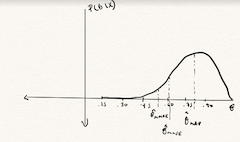
\includegraphics{hw02_2H.png}

\intermediatesubproblem{Show that the posterior is a beta distribution and specify its parameters.}\spc{5}


\hardsubproblem{[MA] Prove that the posterior expectation is the mean squared error optimal estimator given your prior and the data.}\spc{3}

\easysubproblem{Now imagine you are not indifferent and you have some idea about what $\theta$ could be a priori and that subjective feeling can be specified as a beta distribution. (1) Draw the basic shapes that the beta distribution can take on, (2) give an example of $\alpha$ and $\beta$ values that would produce these shapes and (3) write a sentence about what each one means for your prior belief. These shapes are in the notes.}\spc{15}

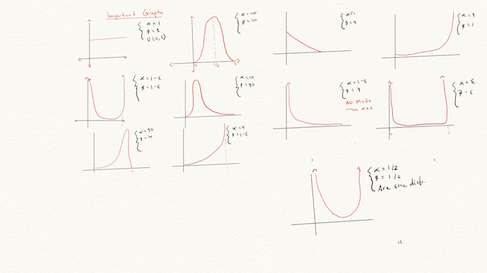
\includegraphics{hw02_2K.png}

\intermediatesubproblem{Imagine $n$ data points of which you don't know the realization values. Using your prior of $\theta \sim \stdbetanot$, show that $\theta~|~X \sim \betanot{\alpha + x}{\beta + (n - x)}$. Note that $x := \sum_{i = 1}^n x_i$ which is the total number of successes and thereby $n-x$ is the total number of failures.}\spc{10}

 If $\theta \sim \stdbetanot$ then,

\begin{align*}
    \prob{\theta | X} \propto \prob{X | \theta} \prob{\theta}
\end{align*}

\begin{align*}
    = {n\choose x}\theta^{x}(1-\theta)^{n-x} \frac{\Gammaf{\alpha +\beta}}{\Gammaf{\alpha}\Gammaf{\beta}\theta^{\alpha -1}(1-\theta)^{\beta-1}}
\end{align*}

\begin{align*}
    = \theta^{x}(1 - \theta)^{n-x}\theta^{\alpha-1}(1-\theta)^{\beta-1}
\end{align*}

\begin{align*}
    \theta^{x+\alpha-1}(1-\theta)^{n-x+\beta-1}
\end{align*}

\begin{align*}
    \prob{\theta|X} = \betanot{\alpha + x}{\beta + n - x}
\end{align*}

\easysubproblem{What does it mean that the beta distribution is the \qu{conjugate prior} for the binomial likelihood?}\spc{3}

It means that if we started with a beta prior, we get a distribution as a posterior.

\hardsubproblem{Show that if $Y \sim \stdbetanot$ then $\var{Y} = \frac{\alpha\beta}{\squared{\alpha + \beta}(\alpha + \beta + 1)}$.}\spc{11}

Recall,

\begin{align*}
    \var{Y} = E(x^{2}) - [(E(x)]^{2} = \int_{0}^{0}{x^{2}f_{x}(x)d\x} - \int_{0}^{1}{x f_{x}(x) d\x}  
\end{align*}

\begin{align*}
    \int_{0}^{1}\frac{x^{\alpha-1}(1-x)^{\beta - 1}}{\betanot{\alpha}{\beta}}d\x - \frac{\alpha^{2}}{(\alpha + \beta) ^2}
\end{align*}

\begin{align*}
    = \frac{\betanot{2 + \alpha}{\beta}}{\betanot{\alpha}{\beta}} - \frac{\alpha^2}{(\alpha + \beta)^2}
 \end{align*}
 
\begin{align*}
   =  \frac{\Gammaf{2 + \alpha} \Gammaf{\beta}}{\Gammaf{2 + \alpha + \beta}} \frac{\Gammaf{\alpha + \beta}}{\Gammaf{\alpha} \Gammaf{\beta}} - \frac{\alpha^2}{(\alpha + \beta)^2} 
\end{align*}

\begin{align*}
    \frac{\alpha(\alpha+1)}{(\alpha+\beta)(\alpha+\beta+1)} - \frac{\alpha^2}{(\alpha + \beta)^2}
\end{align*}

\begin{align*}
  = \frac{\alpha(\alpha+1)(\alpha+\beta) - \alpha^2(\alpha+\beta+1)}{(\alpha + \beta)^2(\alpha+\beta+1)}
\end{align*}

\begin{align*}
    \var{Y} = \frac{\alpha\beta}{(\alpha + \beta)^2(\alpha+\beta+1)}    
\end{align*}


\extracreditsubproblem{Prove that $B(\alpha, \beta) = \frac{\Gammaf{\alpha} \Gammaf{\beta}}{\Gammaf{\alpha + \beta}}$.}

\begin{align*}
    \B(x,y) = \int_{0}^{1}{t^{x-1}(1-t)^{y-1}} = \frac{(x-1)!(y-1)!}{(x+y-1)!}
\end{align*}

\begin{align*}
    \Gammaf{s} = \int_{0}^{\infty}x^{s-1}\exp{-x}d\x
\end{align*}

\begin{align*}
    \Gammaf{m}\Gammaf{n} = \int_{0}^{\infty}x^{m-1}\exp{-x}d\x \int_{0}^{\infty} y^{n-1}\exp{-y}d\y
\end{align*}

\begin{align*}
    = \int_{0}^{\infty}\int_{0}^{\infty}x^{m-1}y^{n-1}\exp{-(x+y)}d\x d\y
\end{align*}

\begin{align*}
   x = v t ,  y = v(1-t)
\end{align*}

\begin{align*}
    =  \int_{0}^{\infty}(v t)^{m-1}(v(1-t))^{n-1}\exp{-(v t + v(1 - t)}d\x d\y
\end{align*}

\begin{align*}
    \Gammaf{m}\Gammaf{n} =  \int_{0}^{\infty} t^{m-1}(1-t)^{n-1}d t  \int_{0}^{\infty}v^{m+n-1}\exp{-v}d v
\end{align*}

\begin{align*}
    \Gammaf{m}\Gammaf{n} = B(m,n)\Gammaf{m+n}
\end{align*}




\intermediatesubproblem{The posterior is $\theta~|~X \sim \betanot{\alpha + x}{\beta + (n - x)}$. Some say the values of $\alpha$ and $\beta$ can be interpreted as follows: $\alpha$ is considered the prior number of successes and $\beta$ is considered the prior number of failures. Why is this a good interpretation? Writing out the PDF of $\theta~|~X$ should help you see it.}\spc{5}

If $\theta$ is considered the prior number of successes and $\beta$ is considered the prior number of failures then anything that is added to each must be the same unit. This is a good interpretation because it is consistent with the way we add the known successes to $\theta$ and the know failure to $\beta$ respectively


\intermediatesubproblem{If you employ the principle of indifference, how many successes and failures is that equivalent to seeing a priori?}\spc{3}

One pseudo success and one pseudo failure. 
\begin{align*}
    U(0,1) = B(1,1)
\end{align*}

\easysubproblem{Why are large values of $\alpha$ and/or $\beta$ considered to compose a \qu{strong} prior?}\spc{2}

$\alpha$ and $\beta$ are pseudo successes and pseudo failure respectively. If $\theta$ and $\beta$ are large then the stronger your belief is. At the end, if you have enough data, the data "swamps the prior" if your prior is weak. 

\intermediatesubproblem{[MA] What is the weakest prior you can think of and why?}\spc{5}

Using a uniform prior because it gives 50/50 odds to each event.

\hardsubproblem{I think a priori that $\theta$ should be expected to be 0.8 with a standard error of 0.02. Solve for the values of $\alpha$ and $\beta$ based on my a priori specification. }\spc{9}

Let $\pi_0$ be expectation and $\sigma^2$ the stardard error, respectively. 

\begin{align*}
    \alpha = \frac{\pi_0(\pi_0(1-\pi_0)- \sigma^2)}{\sigma^2} = \frac{0.8(0.8(1-0.8)-0.02^2)}{0.02^2} = 319.2
\end{align*}

\begin{align*}
    \beta = \frac{\pi_0(1-\pi_0)-\sigma^2}{\sigma^2} - \alpha = \frac{(0.8)(1-0.8)-(0.02)^2}{(0.02)^2} - 319.2 = 79.8
\end{align*}



%\hardsubproblem{Prove that the posterior predictive distribution is $X^*~|~X \sim \bernoulli{\frac{x + \alpha}{n + \alpha + \beta}}$. MA students --- do this yourself. Other students --- use my notes and justify each step. I use a property of the \href{https://en.wikipedia.org/wiki/Gamma_function}{gamma function}. Remember, if $W \sim \bernoulli{\theta}$ then $\prob{W=1} = \theta$. Use that trick! Set $X^* = 1$ and find that probability!}\spc{12}


\easysubproblem{Assume the dataset in (b) where $n=6$. Assume $\theta \sim \betanot{\alpha=2}{\beta=2}$ a priori. Find the $\thetahatmap$, $\thetahatmmse$ and $\thetahatmae$ estimates for $\theta$. For the $\thetahatmae$ estimate, you'll need to obtain a quantile of the beta distribution. Use \texttt{R} on your computer or online using \href{http://rextester.com/l/r_online_compiler}{rextester}. The \texttt{qbeta} function in \texttt{R} finds arbitrary beta quantiles. Its first argument is the quantile desired e.g. 2.5\%, the next is $\alpha$ and the third is $\beta$. So to find the 97.5\%ile of a $\betanot{\alpha=2}{\beta=2}$ for example you type \texttt{qbeta(.975, 2, 2)} into the \texttt{R} console.}\spc{2}

\begin{align*}
    \thetahatmap = \bar{X} = \frac{5}{6} = 0.883
\end{align*}

\begin{align*}
    \thetahatmmse = 
\end{align*}

\intermediatesubproblem{Why are all three of these estimates the same?}\spc{5}

Due to the small size of the dataset

\easysubproblem{Write out an expression for the 95\% credible region for $\theta$. Then write out the answer using the \texttt{qbeta} function from the \texttt{R} language.}\spc{3}

\begin{align*}
    CR_{\theta, 95\%} = [Quantile(2.5\%, 7, 3), Quantile(97.5\%, 7, 3)]
\end{align*}
    
\begin{align*}
    CR_{\theta, 95\%}  = [\texttt{qbeta}(.025, 7 , 3), \texttt{qbeta}(.975, 7 , 3)]
\end{align*}

\easysubproblem{Compute a 95\% frequentist CI for $\theta$.}\spc{5}

\begin{align*}
    CI_{\theta, 95\%} = [0.833 + (1.960)\frac{0.4082}{\sqrt{6}}, 0.833 + (1.960)\frac{0.4082}{\sqrt{6}}] = [0.506, 1.159]
\end{align*}

\hardsubproblem{Let $\mu : \reals \rightarrow \reals^+$ be the \href{https://en.wikipedia.org/wiki/Lebesgue_measure}{Lebesgue measure} which measures the length of a subset of $\reals$. Why is $\mu(\text{CR}) < \mu(\text{CI})$? That is, why is the Bayesian Confidence Interval tighter than the Frequentist Confidence Interval? Use your previous answers. }\spc{5}

Bayesian confidence intervals use the data to construct the interval whereas an Frequentist confidence interval does not take it into consideration and it assumes an asymptotic normality. 

\easysubproblem{Explain the disadvantages of the highest density region method for computing credible regions.}\spc{3}

Highest Density Regions are computationally intense. Additionally, they are non-contiguous as they supply multiple possible locations for $\theta$. 

\intermediatesubproblem{Design a prior where you believe $\expe{\theta} = 0.5$ and you feel as if your belief represents information contained in five coin flips.}\spc{3}

\begin{align*}
    Beta(2.5, 2.5)
\end{align*}
\intermediatesubproblem{Calculate a 95\% a priori credible region for $\theta$. Use \texttt{R} on your computer (or \href{https://rdrr.io/snippets/}{rdrr.io} online) and its \texttt{qbeta} function.}\spc{3}

\begin{align*}
    CR_{\theta, 95\%} = [\texttt{qbeta}(0.025, 2.5, 2.5), \texttt{qbeta}(0.975, 2.5, 2.5)] = [0.123, 0.877]
\end{align*}

\easysubproblem{You flip the same coin 100 times and you observe 39 heads. Calculate a 95\% a posteriori credible region for $\theta$. Round to the nearest 3 decimal points.}\spc{0.5}


If we use the principle of indifference, 
\begin{align*}
    \prob{\theta | X} = Beta(1  +39, 100 - 39 + 1) = Beta(40 , 60) 
\end{align*}

\begin{align*}
    CR_{\theta, 95\%} = [\texttt{qbeta}(0.025, 40, 60), \texttt{qbeta}(0.975, 40, 60)] = [0.307, 0.497]
\end{align*}

\end{enumerate}


\end{document}